\documentclass[journal,12pt,twocolumn]{IEEEtran}
\IEEEoverridecommandlockouts
\usepackage{cite}
\usepackage{amsmath,amssymb,amsfonts,bm}
\usepackage{mathtools}
\usepackage{tkz-euclide} 
\usetikzlibrary{calc,math}
 \usepackage{caption}
\usepackage{listings}
\let\vec\mathbf
\newcommand{\myvec}[1]{\ensuremath{\begin{pmatrix}#1\end{pmatrix}}}
\newcommand{\norm}[1]{\left\lVert#1\right\rVert}
%\lstset{
%frame=single, 
%breaklines=true,
%columns=fullflexible
%}

\begin{document}

\title{Matrix Theory EE5609 - Assignment 3\\
Find if a triangle is isosceles triangle.
}

\author{\IEEEauthorblockN{Sandhya Addetla}\\
\IEEEauthorblockA{PhD Artificial Inteligence Department} \\
23-Sep-2020\\
AI20RESCH14001\\
 }

\maketitle
\begin{abstract}
This document provides a solution for finding if a traingle is isosceles given two equal altitudes of the triangle
\end{abstract}
%
%Download all python codes from 
%\begin{lstlisting}
%https://github.com/SANDHYA-A/Codes/blob/master/Assignment2.py
%\end{lstlisting}


\section{Problem Statement}
BE and CF are two equal altitudes of a triangle ABC. Prove that the triangle ABC is isosceles.


\section{Solution}
Given that BE and CF are two equal altitudes of a triangle ABC.

\captionsetup{justification=centering}

\begin{figure}[!h]
\centering
%\includegraphics[width=0.7\columnwidth]{
\resizebox{.5\columnwidth}{!}{
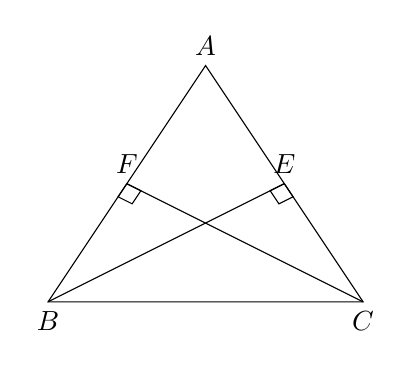
\begin{tikzpicture} 
        \coordinate (A) at (2, 3) {};
        \coordinate (B) at (0, 0) {};
        \coordinate (C) at (4, 0) {};
        \coordinate (F) at (1, 1.5) {};
        \coordinate (E) at (3, 1.5) {};
\draw (A)node[above]{$A$}--(B)node[below]{$B$}--(C)node[below]{$C$}--cycle;
\draw (B)node[below]{}--(E)node[above]{$E$};
\draw (C)node[below]{}--(F)node[above]{$F$};
\tkzMarkRightAngle[size=.2](B,E,C);
\tkzLabelAngle[dist=.5](B,E,C){};
\tkzMarkRightAngle[size=.2](C,F,B);
\tkzLabelAngle[dist=.5](C,F,B){};
\end{tikzpicture}
}
\caption{Triangle with equal altitudes on two sides}
\label{myfig}
\end{figure}
Given that ,
\begin{align}
\norm{\vec{(B-E)} }= \norm{\vec{(C-F)}}\\
\norm{\vec{(B-A)}} + \norm{\vec{(A-E)}} = \norm{\vec{(C-A)}} +\norm{\vec {(A-F)}}
\end{align}
\begin{align}
\begin{aligned}
\norm{\vec{(B-A)}} + \norm{\vec{ (A-B)}} + \norm{\vec{(B-E)}} =\\ \norm{\vec{(C-A)}} +\norm{\vec{ (A-C)}} + \norm{\vec{(C-F)}}
\end{aligned}
\end{align}
\begin{align}
\begin{aligned}
\norm{\vec{(B-A)}} + \norm{\vec{ (A-B)}} =\\ \norm{\vec{(C-A)}} +\norm{\vec{ (A-C)}}
\end{aligned}
\end{align}
\begin{align}
2 \times \norm{\vec{(B-A)}}= 2 \times \norm{\vec{(C-A)}} \\
\norm{\vec{(B-A)}}=\ \norm{\vec{(C-A)}} 
\end{align}
Therefore, the sides  AB and AC of the $\triangle ABC$ are of the same magnitude. Hence $\triangle ABC$ is an isosceles triangle with equal sides AB and AC.
\end{document}